\section*{Βήμα 9}

Πρώτα από όλα κάνουμε clone τα δεδομένα σε μορφή .wav από το repository της εργασίας στον υπολογιστή μας. \\

\noindent Κατόπιν, υλοποιούμε τη συνάρτηση \textit{parse\_free\_digits} προκειμένου να διαβάσουμε σωστά τα αρχεία με τη βιβλιοθήκη librosa.

\lstinputlisting[language=Python, firstline=29, lastline=49]{../../lab.py}

\noindent Το αποτέλεσμα της κλήσης της συνάρτησης είναι:

\begin{center}
	\textbf{Total wavs: 3000. Fs = 8000 Hz}
\end{center}

\noindent Στην συνέχεια βασισμένοι στην υπολοποίηση του βοηθητικού κώδικα ορίζουμε τη δικιά μας συνάρτηση \textit{split\_free\_digits} την οποία παρουσιάζουμε παρακάτω:

\lstinputlisting[language=Python, firstline=52, lastline=85]{../../lab.py}

\noindent Τρέχουμε τον κώδικα για να επιβεβαιώσουμε την ορθή λειτουργία του:

\begin{figure}[H]
	\centering
	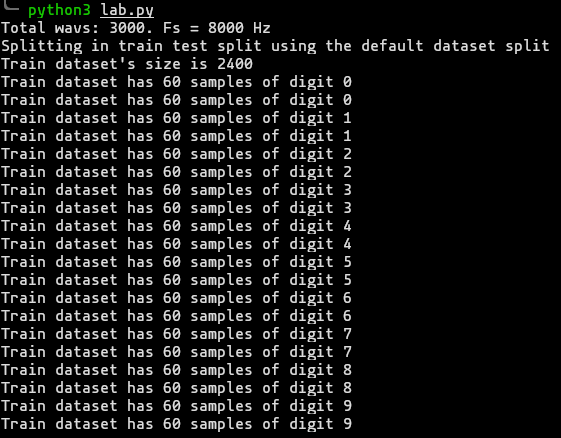
\includegraphics[width=0.5\linewidth]{plots/train_test_res.png}
\end{figure}

\noindent Βλέπουμε ότι το split που έχουμε κάνει έχει μέγεθος 2400, δηλαδή είναι πράγματι το 80\% του 3000. Επιπλέον, είναι ισορροπημένο, αφού υπάρχει ίδιος αριθμός δειγμάτων ήχου σε κάθε κατηγορία - ψηφίο (60). Επομένως ως μετρική του \textit{accuracy} θα είναι αρκετό για να αξιολογήσουμε την επίδοση των ταξινομητών μας (όπως είδαμε και στην προπαρασκευή, στην περίπτωση του ισορροπημένου dataset το F1-score ακολουθεί το ίδιο trend με το accuracy). \\

\noindent Αφού επιβεβαιώσαμε την ορθή λειτουργία της ρουτίνας μας αφαιρούμε - μετατρέπουμε σε σχόλιο τον κώδικα για το debugging.